\documentclass{standalone}
\usepackage{tikz}
\usetikzlibrary{patterns, positioning}


\begin{document}
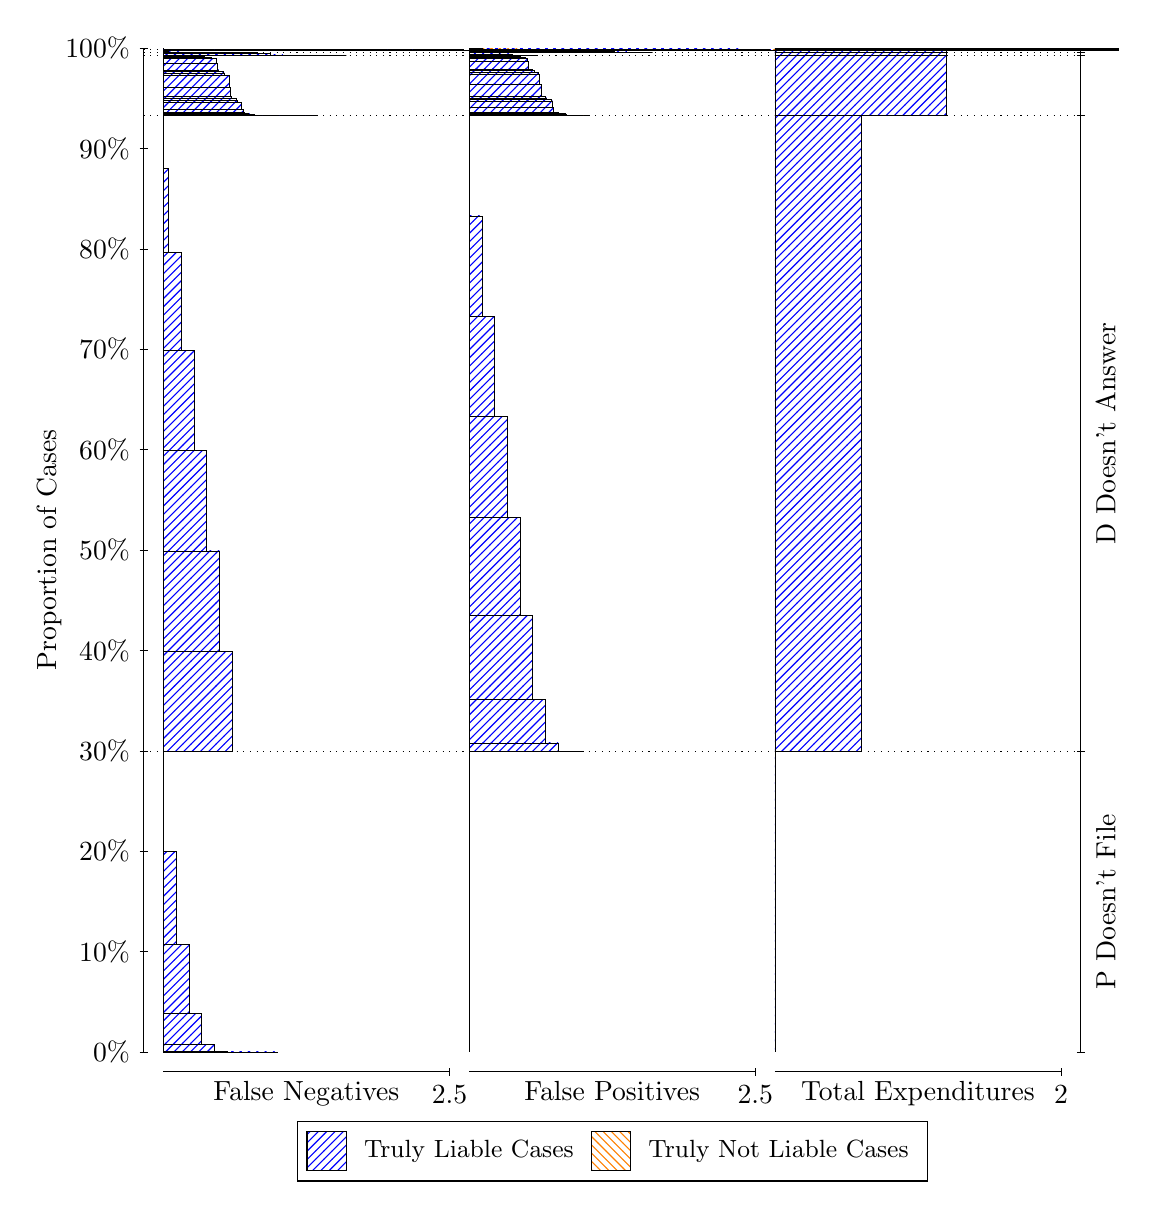
\begin{tikzpicture}
\draw[black, very thin] (1.5,1.75) -- (1.5,14.5);
\node[rotate=90, text=black, anchor=center] at (0.3, 8.125) {Proportion of Cases};
\draw[black, very thin] (1.45,1.75) -- (1.55,1.75);
\node[text=black, anchor=east] at (1.45, 1.75) {0\%};
\draw[black, very thin] (1.45,3.025) -- (1.55,3.025);
\node[text=black, anchor=east] at (1.45, 3.025) {10\%};
\draw[black, very thin] (1.45,4.3) -- (1.55,4.3);
\node[text=black, anchor=east] at (1.45, 4.3) {20\%};
\draw[black, very thin] (1.45,5.575) -- (1.55,5.575);
\node[text=black, anchor=east] at (1.45, 5.575) {30\%};
\draw[black, very thin] (1.45,6.85) -- (1.55,6.85);
\node[text=black, anchor=east] at (1.45, 6.85) {40\%};
\draw[black, very thin] (1.45,8.125) -- (1.55,8.125);
\node[text=black, anchor=east] at (1.45, 8.125) {50\%};
\draw[black, very thin] (1.45,9.4) -- (1.55,9.4);
\node[text=black, anchor=east] at (1.45, 9.4) {60\%};
\draw[black, very thin] (1.45,10.675) -- (1.55,10.675);
\node[text=black, anchor=east] at (1.45, 10.675) {70\%};
\draw[black, very thin] (1.45,11.95) -- (1.55,11.95);
\node[text=black, anchor=east] at (1.45, 11.95) {80\%};
\draw[black, very thin] (1.45,13.225) -- (1.55,13.225);
\node[text=black, anchor=east] at (1.45, 13.225) {90\%};
\draw[black, very thin] (1.45,14.5) -- (1.55,14.5);
\node[text=black, anchor=east] at (1.45, 14.5) {100\%};

\draw[black, very thin] (13.4,1.75) -- (13.4,14.5);
\draw[black, very thin] (13.35,1.75) -- (13.45,1.75);
\node[anchor=west] at (13.35, 1.75) {};
\draw[black, very thin] (13.35,5.563) -- (13.45,5.563);
\node[anchor=west] at (13.35, 5.563) {};
\draw[black, very thin] (13.35,13.642) -- (13.45,13.642);
\node[anchor=west] at (13.35, 13.642) {};
\draw[black, very thin] (13.35,14.408) -- (13.45,14.408);
\node[anchor=west] at (13.35, 14.408) {};
\draw[black, very thin] (13.35,14.447) -- (13.45,14.447);
\node[anchor=west] at (13.35, 14.447) {};
\draw[black, very thin] (13.35,14.476) -- (13.45,14.476);
\node[anchor=west] at (13.35, 14.476) {};
\draw[black, very thin] (13.35,14.5) -- (13.45,14.5);
\node[anchor=west] at (13.35, 14.5) {};

\draw[black, very thin, pattern color=blue, pattern=north east lines] (1.75,1.75) rectangle (3.2033,1.75);
\draw[black, very thin, pattern color=blue, pattern=north east lines] (1.75,1.75) rectangle (3.0419,1.75);
\draw[black, very thin, pattern color=blue, pattern=north east lines] (1.75,1.75) rectangle (2.8804,1.75);
\draw[black, very thin, pattern color=blue, pattern=north east lines] (1.75,1.75) rectangle (2.7189,1.7503);
\draw[black, very thin, pattern color=blue, pattern=north east lines] (1.75,1.7503) rectangle (2.5574,1.7582);
\draw[black, very thin, pattern color=blue, pattern=north east lines] (1.75,1.7582) rectangle (2.3959,1.8434);
\draw[black, very thin, pattern color=blue, pattern=north east lines] (1.75,1.8434) rectangle (2.2344,2.2366);
\draw[black, very thin, pattern color=blue, pattern=north east lines] (1.75,2.2366) rectangle (2.073,3.1157);
\draw[black, very thin, pattern color=blue, pattern=north east lines] (1.75,3.1157) rectangle (1.9115,4.2995);
\draw[black, very thin, pattern color=orange, pattern=north west lines] (1.75,4.2995) rectangle (1.75,4.2995);
\draw[black, very thin, pattern color=blue, pattern=north east lines] (1.75,4.2995) rectangle (1.75,5.563);
\draw[black, very thin, pattern color=blue, pattern=north east lines] (1.75,5.563) rectangle (2.622,6.838);
\draw[black, very thin, pattern color=blue, pattern=north east lines] (1.75,6.838) rectangle (2.4605,8.113);
\draw[black, very thin, pattern color=blue, pattern=north east lines] (1.75,8.113) rectangle (2.299,9.388);
\draw[black, very thin, pattern color=blue, pattern=north east lines] (1.75,9.388) rectangle (2.1376,10.661);
\draw[black, very thin, pattern color=blue, pattern=north east lines] (1.75,10.661) rectangle (1.9761,11.908);
\draw[black, very thin, pattern color=blue, pattern=north east lines] (1.75,11.908) rectangle (1.8146,12.973);
\draw[black, very thin, pattern color=orange, pattern=north west lines] (1.75,12.973) rectangle (1.75,12.973);
\draw[black, very thin, pattern color=blue, pattern=north east lines] (1.75,12.973) rectangle (1.75,13.642);
\draw[black, very thin, pattern color=blue, pattern=north east lines] (1.75,13.642) rectangle (3.712,13.642);
\draw[black, very thin, pattern color=blue, pattern=north east lines] (1.75,13.642) rectangle (3.6393,13.642);
\draw[black, very thin, pattern color=blue, pattern=north east lines] (1.75,13.642) rectangle (3.5667,13.642);
\draw[black, very thin, pattern color=blue, pattern=north east lines] (1.75,13.642) rectangle (3.5505,13.642);
\draw[black, very thin, pattern color=blue, pattern=north east lines] (1.75,13.642) rectangle (3.494,13.642);
\draw[black, very thin, pattern color=blue, pattern=north east lines] (1.75,13.642) rectangle (3.4779,13.642);
\draw[black, very thin, pattern color=blue, pattern=north east lines] (1.75,13.642) rectangle (3.4213,13.642);
\draw[black, very thin, pattern color=blue, pattern=north east lines] (1.75,13.642) rectangle (3.4052,13.642);
\draw[black, very thin, pattern color=blue, pattern=north east lines] (1.75,13.642) rectangle (3.389,13.642);
\draw[black, very thin, pattern color=blue, pattern=north east lines] (1.75,13.642) rectangle (3.3325,13.642);
\draw[black, very thin, pattern color=blue, pattern=north east lines] (1.75,13.642) rectangle (3.3164,13.642);
\draw[black, very thin, pattern color=blue, pattern=north east lines] (1.75,13.642) rectangle (3.2599,13.642);
\draw[black, very thin, pattern color=blue, pattern=north east lines] (1.75,13.642) rectangle (3.2437,13.642);
\draw[black, very thin, pattern color=blue, pattern=north east lines] (1.75,13.642) rectangle (3.2276,13.642);
\draw[black, very thin, pattern color=blue, pattern=north east lines] (1.75,13.642) rectangle (3.171,13.642);
\draw[black, very thin, pattern color=blue, pattern=north east lines] (1.75,13.642) rectangle (3.1549,13.642);
\draw[black, very thin, pattern color=blue, pattern=north east lines] (1.75,13.642) rectangle (3.0984,13.642);
\draw[black, very thin, pattern color=blue, pattern=north east lines] (1.75,13.642) rectangle (3.0822,13.642);
\draw[black, very thin, pattern color=blue, pattern=north east lines] (1.75,13.642) rectangle (3.0661,13.643);
\draw[black, very thin, pattern color=blue, pattern=north east lines] (1.75,13.643) rectangle (3.0096,13.643);
\draw[black, very thin, pattern color=blue, pattern=north east lines] (1.75,13.643) rectangle (2.9934,13.643);
\draw[black, very thin, pattern color=blue, pattern=north east lines] (1.75,13.643) rectangle (2.9369,13.644);
\draw[black, very thin, pattern color=blue, pattern=north east lines] (1.75,13.644) rectangle (2.9207,13.647);
\draw[black, very thin, pattern color=blue, pattern=north east lines] (1.75,13.647) rectangle (2.9046,13.662);
\draw[black, very thin, pattern color=blue, pattern=north east lines] (1.75,13.662) rectangle (2.8481,13.665);
\draw[black, very thin, pattern color=blue, pattern=north east lines] (1.75,13.665) rectangle (2.8319,13.671);
\draw[black, very thin, pattern color=blue, pattern=north east lines] (1.75,13.671) rectangle (2.7754,13.678);
\draw[black, very thin, pattern color=blue, pattern=north east lines] (1.75,13.678) rectangle (2.7593,13.719);
\draw[black, very thin, pattern color=blue, pattern=north east lines] (1.75,13.719) rectangle (2.7431,13.815);
\draw[black, very thin, pattern color=blue, pattern=north east lines] (1.75,13.815) rectangle (2.6866,13.835);
\draw[black, very thin, pattern color=blue, pattern=north east lines] (1.75,13.835) rectangle (2.6704,13.861);
\draw[black, very thin, pattern color=blue, pattern=north east lines] (1.75,13.861) rectangle (2.6139,13.881);
\draw[black, very thin, pattern color=blue, pattern=north east lines] (1.75,13.881) rectangle (2.5978,14.005);
\draw[black, very thin, pattern color=blue, pattern=north east lines] (1.75,14.005) rectangle (2.5816,14.157);
\draw[black, very thin, pattern color=blue, pattern=north east lines] (1.75,14.157) rectangle (2.5251,14.185);
\draw[black, very thin, pattern color=blue, pattern=north east lines] (1.75,14.185) rectangle (2.509,14.207);
\draw[black, very thin, pattern color=blue, pattern=north east lines] (1.75,14.207) rectangle (2.4524,14.221);
\draw[black, very thin, pattern color=blue, pattern=north east lines] (1.75,14.221) rectangle (2.4363,14.304);
\draw[black, very thin, pattern color=blue, pattern=north east lines] (1.75,14.304) rectangle (2.4201,14.37);
\draw[black, very thin, pattern color=blue, pattern=north east lines] (1.75,14.37) rectangle (2.3636,14.378);
\draw[black, very thin, pattern color=blue, pattern=north east lines] (1.75,14.378) rectangle (2.3475,14.382);
\draw[black, very thin, pattern color=blue, pattern=north east lines] (1.75,14.382) rectangle (2.291,14.384);
\draw[black, very thin, pattern color=blue, pattern=north east lines] (1.75,14.384) rectangle (2.2748,14.396);
\draw[black, very thin, pattern color=blue, pattern=north east lines] (1.75,14.396) rectangle (2.2587,14.407);
\draw[black, very thin, pattern color=blue, pattern=north east lines] (1.75,14.407) rectangle (2.2021,14.407);
\draw[black, very thin, pattern color=blue, pattern=north east lines] (1.75,14.407) rectangle (2.186,14.408);
\draw[black, very thin, pattern color=blue, pattern=north east lines] (1.75,14.408) rectangle (2.1295,14.408);
\draw[black, very thin, pattern color=blue, pattern=north east lines] (1.75,14.408) rectangle (2.1133,14.408);
\draw[black, very thin, pattern color=blue, pattern=north east lines] (1.75,14.408) rectangle (2.0407,14.408);
\draw[black, very thin, pattern color=blue, pattern=north east lines] (1.75,14.408) rectangle (1.968,14.408);
\draw[black, very thin, pattern color=orange, pattern=north west lines] (1.75,14.408) rectangle (1.75,14.408);
\draw[black, very thin, pattern color=blue, pattern=north east lines] (1.75,14.408) rectangle (4.0753,14.408);
\draw[black, very thin, pattern color=blue, pattern=north east lines] (1.75,14.408) rectangle (3.9139,14.408);
\draw[black, very thin, pattern color=blue, pattern=north east lines] (1.75,14.408) rectangle (3.7524,14.408);
\draw[black, very thin, pattern color=blue, pattern=north east lines] (1.75,14.408) rectangle (3.5909,14.408);
\draw[black, very thin, pattern color=blue, pattern=north east lines] (1.75,14.408) rectangle (3.4294,14.408);
\draw[black, very thin, pattern color=blue, pattern=north east lines] (1.75,14.408) rectangle (3.2679,14.413);
\draw[black, very thin, pattern color=blue, pattern=north east lines] (1.75,14.413) rectangle (3.1064,14.43);
\draw[black, very thin, pattern color=blue, pattern=north east lines] (1.75,14.43) rectangle (2.945,14.444);
\draw[black, very thin, pattern color=blue, pattern=north east lines] (1.75,14.444) rectangle (2.7835,14.447);
\draw[black, very thin, pattern color=blue, pattern=north east lines] (1.75,14.447) rectangle (2.622,14.447);
\draw[black, very thin, pattern color=orange, pattern=north west lines] (1.75,14.447) rectangle (1.75,14.447);
\draw[black, very thin, pattern color=blue, pattern=north east lines] (1.75,14.447) rectangle (2.622,14.447);
\draw[black, very thin, pattern color=blue, pattern=north east lines] (1.75,14.447) rectangle (2.4605,14.447);
\draw[black, very thin, pattern color=blue, pattern=north east lines] (1.75,14.447) rectangle (2.299,14.447);
\draw[black, very thin, pattern color=blue, pattern=north east lines] (1.75,14.447) rectangle (2.1376,14.448);
\draw[black, very thin, pattern color=blue, pattern=north east lines] (1.75,14.448) rectangle (1.9761,14.452);
\draw[black, very thin, pattern color=blue, pattern=north east lines] (1.75,14.452) rectangle (1.8146,14.462);
\draw[black, very thin, pattern color=orange, pattern=north west lines] (1.75,14.462) rectangle (1.75,14.462);
\draw[black, very thin, pattern color=blue, pattern=north east lines] (1.75,14.462) rectangle (1.75,14.476);
\draw[black, very thin, pattern color=blue, pattern=north east lines] (1.75,14.476) rectangle (6.6913,14.476);
\draw[black, very thin, pattern color=blue, pattern=north east lines] (1.75,14.476) rectangle (6.5299,14.476);
\draw[black, very thin, pattern color=blue, pattern=north east lines] (1.75,14.476) rectangle (6.3684,14.476);
\draw[black, very thin, pattern color=blue, pattern=north east lines] (1.75,14.476) rectangle (6.2069,14.476);
\draw[black, very thin, pattern color=blue, pattern=north east lines] (1.75,14.476) rectangle (6.0454,14.476);
\draw[black, very thin, pattern color=blue, pattern=north east lines] (1.75,14.476) rectangle (6.0454,14.476);
\draw[black, very thin, pattern color=blue, pattern=north east lines] (1.75,14.476) rectangle (5.8839,14.476);
\draw[black, very thin, pattern color=blue, pattern=north east lines] (1.75,14.476) rectangle (5.7224,14.477);
\draw[black, very thin, pattern color=blue, pattern=north east lines] (1.75,14.477) rectangle (5.7224,14.477);
\draw[black, very thin, pattern color=blue, pattern=north east lines] (1.75,14.477) rectangle (5.561,14.479);
\draw[black, very thin, pattern color=blue, pattern=north east lines] (1.75,14.479) rectangle (5.561,14.48);
\draw[black, very thin, pattern color=blue, pattern=north east lines] (1.75,14.48) rectangle (5.3995,14.484);
\draw[black, very thin, pattern color=blue, pattern=north east lines] (1.75,14.484) rectangle (5.238,14.486);
\draw[black, very thin, pattern color=blue, pattern=north east lines] (1.75,14.486) rectangle (5.0765,14.486);
\draw[black, very thin, pattern color=blue, pattern=north east lines] (1.75,14.486) rectangle (4.915,14.486);
\draw[black, very thin, pattern color=blue, pattern=north east lines] (1.75,14.486) rectangle (4.7536,14.486);
\draw[black, very thin, pattern color=blue, pattern=north east lines] (1.75,14.486) rectangle (4.5921,14.486);
\draw[black, very thin, pattern color=blue, pattern=north east lines] (1.75,14.486) rectangle (2.7189,14.486);
\draw[black, very thin, pattern color=blue, pattern=north east lines] (1.75,14.486) rectangle (2.5574,14.486);
\draw[black, very thin, pattern color=blue, pattern=north east lines] (1.75,14.486) rectangle (2.3959,14.486);
\draw[black, very thin, pattern color=blue, pattern=north east lines] (1.75,14.486) rectangle (2.3959,14.486);
\draw[black, very thin, pattern color=blue, pattern=north east lines] (1.75,14.486) rectangle (2.2344,14.486);
\draw[black, very thin, pattern color=blue, pattern=north east lines] (1.75,14.486) rectangle (2.2344,14.486);
\draw[black, very thin, pattern color=blue, pattern=north east lines] (1.75,14.486) rectangle (2.2344,14.486);
\draw[black, very thin, pattern color=blue, pattern=north east lines] (1.75,14.486) rectangle (2.073,14.486);
\draw[black, very thin, pattern color=blue, pattern=north east lines] (1.75,14.486) rectangle (2.073,14.486);
\draw[black, very thin, pattern color=blue, pattern=north east lines] (1.75,14.486) rectangle (1.9115,14.486);
\draw[black, very thin, pattern color=blue, pattern=north east lines] (1.75,14.486) rectangle (1.9115,14.487);
\draw[black, very thin, pattern color=blue, pattern=north east lines] (1.75,14.487) rectangle (1.9115,14.487);
\draw[black, very thin, pattern color=orange, pattern=north west lines] (1.75,14.487) rectangle (1.75,14.487);
\draw[black, very thin, pattern color=blue, pattern=north east lines] (1.75,14.487) rectangle (1.75,14.5);
\draw[black, very thin, pattern color=orange, pattern=north west lines] (5.6333,1.75) rectangle (5.6333,1.75);
\draw[black, very thin, pattern color=blue, pattern=north east lines] (5.6333,1.75) rectangle (5.6333,5.563);
\draw[black, very thin, pattern color=orange, pattern=north west lines] (5.6333,5.563) rectangle (7.0867,5.563);
\draw[black, very thin, pattern color=blue, pattern=north east lines] (5.6333,5.563) rectangle (7.0867,5.5631);
\draw[black, very thin, pattern color=blue, pattern=north east lines] (5.6333,5.5631) rectangle (6.9252,5.5687);
\draw[black, very thin, pattern color=blue, pattern=north east lines] (5.6333,5.5687) rectangle (6.7637,5.6763);
\draw[black, very thin, pattern color=blue, pattern=north east lines] (5.6333,5.6763) rectangle (6.6022,6.2324);
\draw[black, very thin, pattern color=blue, pattern=north east lines] (5.6333,6.2324) rectangle (6.4407,7.297);
\draw[black, very thin, pattern color=blue, pattern=north east lines] (5.6333,7.297) rectangle (6.2793,8.5439);
\draw[black, very thin, pattern color=blue, pattern=north east lines] (5.6333,8.5439) rectangle (6.1178,9.8171);
\draw[black, very thin, pattern color=blue, pattern=north east lines] (5.6333,9.8171) rectangle (5.9563,11.092);
\draw[black, very thin, pattern color=blue, pattern=north east lines] (5.6333,11.092) rectangle (5.7948,12.367);
\draw[black, very thin, pattern color=blue, pattern=north east lines] (5.6333,12.367) rectangle (5.6333,13.642);
\draw[black, very thin, pattern color=orange, pattern=north west lines] (5.6333,13.642) rectangle (7.1593,13.642);
\draw[black, very thin, pattern color=blue, pattern=north east lines] (5.6333,13.642) rectangle (7.1593,13.642);
\draw[black, very thin, pattern color=orange, pattern=north west lines] (5.6333,13.642) rectangle (7.0867,13.642);
\draw[black, very thin, pattern color=blue, pattern=north east lines] (5.6333,13.642) rectangle (7.0867,13.642);
\draw[black, very thin, pattern color=orange, pattern=north west lines] (5.6333,13.642) rectangle (7.014,13.642);
\draw[black, very thin, pattern color=blue, pattern=north east lines] (5.6333,13.642) rectangle (7.014,13.643);
\draw[black, very thin, pattern color=blue, pattern=north east lines] (5.6333,13.643) rectangle (6.9979,13.643);
\draw[black, very thin, pattern color=orange, pattern=north west lines] (5.6333,13.643) rectangle (6.9413,13.643);
\draw[black, very thin, pattern color=blue, pattern=north east lines] (5.6333,13.643) rectangle (6.9413,13.643);
\draw[black, very thin, pattern color=blue, pattern=north east lines] (5.6333,13.643) rectangle (6.9252,13.643);
\draw[black, very thin, pattern color=orange, pattern=north west lines] (5.6333,13.643) rectangle (6.8687,13.643);
\draw[black, very thin, pattern color=blue, pattern=north east lines] (5.6333,13.643) rectangle (6.8687,13.654);
\draw[black, very thin, pattern color=blue, pattern=north east lines] (5.6333,13.654) rectangle (6.8525,13.666);
\draw[black, very thin, pattern color=blue, pattern=north east lines] (5.6333,13.666) rectangle (6.8364,13.668);
\draw[black, very thin, pattern color=blue, pattern=north east lines] (5.6333,13.668) rectangle (6.7799,13.672);
\draw[black, very thin, pattern color=blue, pattern=north east lines] (5.6333,13.672) rectangle (6.7637,13.68);
\draw[black, very thin, pattern color=blue, pattern=north east lines] (5.6333,13.68) rectangle (6.7072,13.746);
\draw[black, very thin, pattern color=blue, pattern=north east lines] (5.6333,13.746) rectangle (6.691,13.829);
\draw[black, very thin, pattern color=blue, pattern=north east lines] (5.6333,13.829) rectangle (6.6749,13.843);
\draw[black, very thin, pattern color=blue, pattern=north east lines] (5.6333,13.843) rectangle (6.6184,13.866);
\draw[black, very thin, pattern color=blue, pattern=north east lines] (5.6333,13.866) rectangle (6.6022,13.893);
\draw[black, very thin, pattern color=blue, pattern=north east lines] (5.6333,13.893) rectangle (6.5457,14.045);
\draw[black, very thin, pattern color=blue, pattern=north east lines] (5.6333,14.045) rectangle (6.5296,14.169);
\draw[black, very thin, pattern color=blue, pattern=north east lines] (5.6333,14.169) rectangle (6.5134,14.189);
\draw[black, very thin, pattern color=blue, pattern=north east lines] (5.6333,14.189) rectangle (6.4569,14.215);
\draw[black, very thin, pattern color=blue, pattern=north east lines] (5.6333,14.215) rectangle (6.4407,14.235);
\draw[black, very thin, pattern color=blue, pattern=north east lines] (5.6333,14.235) rectangle (6.3842,14.331);
\draw[black, very thin, pattern color=blue, pattern=north east lines] (5.6333,14.331) rectangle (6.3681,14.373);
\draw[black, very thin, pattern color=blue, pattern=north east lines] (5.6333,14.373) rectangle (6.3519,14.38);
\draw[black, very thin, pattern color=blue, pattern=north east lines] (5.6333,14.38) rectangle (6.2954,14.385);
\draw[black, very thin, pattern color=blue, pattern=north east lines] (5.6333,14.385) rectangle (6.2793,14.389);
\draw[black, very thin, pattern color=blue, pattern=north east lines] (5.6333,14.389) rectangle (6.2227,14.403);
\draw[black, very thin, pattern color=blue, pattern=north east lines] (5.6333,14.403) rectangle (6.2066,14.407);
\draw[black, very thin, pattern color=blue, pattern=north east lines] (5.6333,14.407) rectangle (6.1904,14.407);
\draw[black, very thin, pattern color=blue, pattern=north east lines] (5.6333,14.407) rectangle (6.1339,14.408);
\draw[black, very thin, pattern color=blue, pattern=north east lines] (5.6333,14.408) rectangle (6.1178,14.408);
\draw[black, very thin, pattern color=blue, pattern=north east lines] (5.6333,14.408) rectangle (6.0613,14.408);
\draw[black, very thin, pattern color=blue, pattern=north east lines] (5.6333,14.408) rectangle (6.0451,14.408);
\draw[black, very thin, pattern color=blue, pattern=north east lines] (5.6333,14.408) rectangle (6.029,14.408);
\draw[black, very thin, pattern color=blue, pattern=north east lines] (5.6333,14.408) rectangle (5.9724,14.408);
\draw[black, very thin, pattern color=blue, pattern=north east lines] (5.6333,14.408) rectangle (5.9563,14.408);
\draw[black, very thin, pattern color=blue, pattern=north east lines] (5.6333,14.408) rectangle (5.8998,14.408);
\draw[black, very thin, pattern color=blue, pattern=north east lines] (5.6333,14.408) rectangle (5.8836,14.408);
\draw[black, very thin, pattern color=blue, pattern=north east lines] (5.6333,14.408) rectangle (5.8675,14.408);
\draw[black, very thin, pattern color=blue, pattern=north east lines] (5.6333,14.408) rectangle (5.811,14.408);
\draw[black, very thin, pattern color=blue, pattern=north east lines] (5.6333,14.408) rectangle (5.7948,14.408);
\draw[black, very thin, pattern color=blue, pattern=north east lines] (5.6333,14.408) rectangle (5.7383,14.408);
\draw[black, very thin, pattern color=blue, pattern=north east lines] (5.6333,14.408) rectangle (5.7221,14.408);
\draw[black, very thin, pattern color=blue, pattern=north east lines] (5.6333,14.408) rectangle (5.706,14.408);
\draw[black, very thin, pattern color=blue, pattern=north east lines] (5.6333,14.408) rectangle (5.6495,14.408);
\draw[black, very thin, pattern color=blue, pattern=north east lines] (5.6333,14.408) rectangle (5.6333,14.408);
\draw[black, very thin, pattern color=orange, pattern=north west lines] (5.6333,14.408) rectangle (6.5053,14.408);
\draw[black, very thin, pattern color=blue, pattern=north east lines] (5.6333,14.408) rectangle (6.5053,14.408);
\draw[black, very thin, pattern color=blue, pattern=north east lines] (5.6333,14.408) rectangle (6.3439,14.411);
\draw[black, very thin, pattern color=blue, pattern=north east lines] (5.6333,14.411) rectangle (6.1824,14.425);
\draw[black, very thin, pattern color=blue, pattern=north east lines] (5.6333,14.425) rectangle (6.0209,14.443);
\draw[black, very thin, pattern color=blue, pattern=north east lines] (5.6333,14.443) rectangle (5.8594,14.447);
\draw[black, very thin, pattern color=blue, pattern=north east lines] (5.6333,14.447) rectangle (5.6979,14.447);
\draw[black, very thin, pattern color=blue, pattern=north east lines] (5.6333,14.447) rectangle (5.6333,14.447);
\draw[black, very thin, pattern color=orange, pattern=north west lines] (5.6333,14.447) rectangle (7.9587,14.447);
\draw[black, very thin, pattern color=blue, pattern=north east lines] (5.6333,14.447) rectangle (7.9587,14.447);
\draw[black, very thin, pattern color=blue, pattern=north east lines] (5.6333,14.447) rectangle (7.7972,14.447);
\draw[black, very thin, pattern color=blue, pattern=north east lines] (5.6333,14.447) rectangle (7.6357,14.45);
\draw[black, very thin, pattern color=blue, pattern=north east lines] (5.6333,14.45) rectangle (7.4742,14.461);
\draw[black, very thin, pattern color=blue, pattern=north east lines] (5.6333,14.461) rectangle (7.3127,14.472);
\draw[black, very thin, pattern color=blue, pattern=north east lines] (5.6333,14.472) rectangle (7.1513,14.476);
\draw[black, very thin, pattern color=blue, pattern=north east lines] (5.6333,14.476) rectangle (6.9898,14.476);
\draw[black, very thin, pattern color=blue, pattern=north east lines] (5.6333,14.476) rectangle (6.8283,14.476);
\draw[black, very thin, pattern color=blue, pattern=north east lines] (5.6333,14.476) rectangle (6.6668,14.476);
\draw[black, very thin, pattern color=blue, pattern=north east lines] (5.6333,14.476) rectangle (6.5053,14.476);
\draw[black, very thin, pattern color=orange, pattern=north west lines] (5.6333,14.476) rectangle (10.575,14.476);
\draw[black, very thin, pattern color=blue, pattern=north east lines] (5.6333,14.476) rectangle (10.575,14.476);
\draw[black, very thin, pattern color=orange, pattern=north west lines] (5.6333,14.476) rectangle (10.413,14.476);
\draw[black, very thin, pattern color=blue, pattern=north east lines] (5.6333,14.476) rectangle (10.413,14.476);
\draw[black, very thin, pattern color=orange, pattern=north west lines] (5.6333,14.476) rectangle (10.252,14.476);
\draw[black, very thin, pattern color=blue, pattern=north east lines] (5.6333,14.476) rectangle (10.252,14.476);
\draw[black, very thin, pattern color=orange, pattern=north west lines] (5.6333,14.476) rectangle (10.09,14.476);
\draw[black, very thin, pattern color=blue, pattern=north east lines] (5.6333,14.476) rectangle (10.09,14.476);
\draw[black, very thin, pattern color=orange, pattern=north west lines] (5.6333,14.476) rectangle (9.9287,14.476);
\draw[black, very thin, pattern color=blue, pattern=north east lines] (5.6333,14.476) rectangle (9.9287,14.476);
\draw[black, very thin, pattern color=blue, pattern=north east lines] (5.6333,14.476) rectangle (9.9287,14.476);
\draw[black, very thin, pattern color=blue, pattern=north east lines] (5.6333,14.476) rectangle (9.7673,14.476);
\draw[black, very thin, pattern color=orange, pattern=north west lines] (5.6333,14.476) rectangle (9.7673,14.476);
\draw[black, very thin, pattern color=blue, pattern=north east lines] (5.6333,14.476) rectangle (9.7673,14.477);
\draw[black, very thin, pattern color=orange, pattern=north west lines] (5.6333,14.477) rectangle (9.6058,14.477);
\draw[black, very thin, pattern color=blue, pattern=north east lines] (5.6333,14.477) rectangle (9.6058,14.477);
\draw[black, very thin, pattern color=blue, pattern=north east lines] (5.6333,14.477) rectangle (9.6058,14.477);
\draw[black, very thin, pattern color=blue, pattern=north east lines] (5.6333,14.477) rectangle (9.4443,14.479);
\draw[black, very thin, pattern color=blue, pattern=north east lines] (5.6333,14.479) rectangle (9.4443,14.48);
\draw[black, very thin, pattern color=blue, pattern=north east lines] (5.6333,14.48) rectangle (9.2828,14.483);
\draw[black, very thin, pattern color=blue, pattern=north east lines] (5.6333,14.483) rectangle (9.2828,14.485);
\draw[black, very thin, pattern color=blue, pattern=north east lines] (5.6333,14.485) rectangle (9.1213,14.485);
\draw[black, very thin, pattern color=blue, pattern=north east lines] (5.6333,14.485) rectangle (9.1213,14.487);
\draw[black, very thin, pattern color=blue, pattern=north east lines] (5.6333,14.487) rectangle (9.1213,14.489);
\draw[black, very thin, pattern color=blue, pattern=north east lines] (5.6333,14.489) rectangle (8.9599,14.489);
\draw[black, very thin, pattern color=blue, pattern=north east lines] (5.6333,14.489) rectangle (8.9599,14.49);
\draw[black, very thin, pattern color=blue, pattern=north east lines] (5.6333,14.49) rectangle (8.7984,14.49);
\draw[black, very thin, pattern color=blue, pattern=north east lines] (5.6333,14.49) rectangle (8.7984,14.49);
\draw[black, very thin, pattern color=blue, pattern=north east lines] (5.6333,14.49) rectangle (8.6369,14.49);
\draw[black, very thin, pattern color=blue, pattern=north east lines] (5.6333,14.49) rectangle (8.6369,14.49);
\draw[black, very thin, pattern color=blue, pattern=north east lines] (5.6333,14.49) rectangle (8.4754,14.49);
\draw[black, very thin, pattern color=blue, pattern=north east lines] (5.6333,14.49) rectangle (8.4754,14.49);
\draw[black, very thin, pattern color=blue, pattern=north east lines] (5.6333,14.49) rectangle (8.3139,14.49);
\draw[black, very thin, pattern color=blue, pattern=north east lines] (5.6333,14.49) rectangle (8.3139,14.49);
\draw[black, very thin, pattern color=blue, pattern=north east lines] (5.6333,14.49) rectangle (8.1524,14.49);
\draw[black, very thin, pattern color=orange, pattern=north west lines] (5.6333,14.49) rectangle (6.2793,14.49);
\draw[black, very thin, pattern color=blue, pattern=north east lines] (5.6333,14.49) rectangle (6.2793,14.49);
\draw[black, very thin, pattern color=orange, pattern=north west lines] (5.6333,14.49) rectangle (6.1178,14.49);
\draw[black, very thin, pattern color=blue, pattern=north east lines] (5.6333,14.49) rectangle (6.1178,14.49);
\draw[black, very thin, pattern color=orange, pattern=north west lines] (5.6333,14.49) rectangle (5.9563,14.49);
\draw[black, very thin, pattern color=blue, pattern=north east lines] (5.6333,14.49) rectangle (5.9563,14.49);
\draw[black, very thin, pattern color=orange, pattern=north west lines] (5.6333,14.49) rectangle (5.7948,14.49);
\draw[black, very thin, pattern color=blue, pattern=north east lines] (5.6333,14.49) rectangle (5.7948,14.491);
\draw[black, very thin, pattern color=orange, pattern=north west lines] (5.6333,14.491) rectangle (5.6333,14.491);
\draw[black, very thin, pattern color=blue, pattern=north east lines] (5.6333,14.491) rectangle (5.6333,14.5);
\draw[black, very thin, pattern color=orange, pattern=north west lines] (9.5167,1.75) rectangle (9.5167,1.75);
\draw[black, very thin, pattern color=blue, pattern=north east lines] (9.5167,1.75) rectangle (9.5167,5.563);
\draw[black, very thin, pattern color=orange, pattern=north west lines] (9.5167,5.563) rectangle (10.607,5.563);
\draw[black, very thin, pattern color=blue, pattern=north east lines] (9.5167,5.563) rectangle (10.607,13.642);
\draw[black, very thin, pattern color=orange, pattern=north west lines] (9.5167,13.642) rectangle (11.697,13.642);
\draw[black, very thin, pattern color=blue, pattern=north east lines] (9.5167,13.642) rectangle (11.697,14.408);
\draw[black, very thin, pattern color=orange, pattern=north west lines] (9.5167,14.408) rectangle (11.697,14.408);
\draw[black, very thin, pattern color=blue, pattern=north east lines] (9.5167,14.408) rectangle (11.697,14.447);
\draw[black, very thin, pattern color=orange, pattern=north west lines] (9.5167,14.447) rectangle (11.697,14.447);
\draw[black, very thin, pattern color=blue, pattern=north east lines] (9.5167,14.447) rectangle (11.697,14.476);
\draw[black, very thin, pattern color=orange, pattern=north west lines] (9.5167,14.476) rectangle (13.877,14.476);
\draw[black, very thin, pattern color=blue, pattern=north east lines] (9.5167,14.476) rectangle (13.877,14.48);
\draw[black, very thin, pattern color=orange, pattern=north west lines] (9.5167,14.48) rectangle (13.877,14.48);
\draw[black, very thin, pattern color=blue, pattern=north east lines] (9.5167,14.48) rectangle (13.877,14.496);
\draw[black, very thin, pattern color=orange, pattern=north west lines] (9.5167,14.496) rectangle (13.877,14.496);
\draw[black, very thin, pattern color=blue, pattern=north east lines] (9.5167,14.496) rectangle (13.877,14.5);
\draw[black, dotted] (1.5,5.563) -- (13.4,5.563);
\draw[black, dotted] (1.5,13.642) -- (13.4,13.642);
\draw[black, dotted] (1.5,14.408) -- (13.4,14.408);
\draw[black, dotted] (1.5,14.447) -- (13.4,14.447);
\draw[black, dotted] (1.5,14.476) -- (13.4,14.476);
\draw[black, very thin] (1.75,1.5) -- (5.3833,1.5);
\node[text=black, anchor=north] at (3.5667, 1.5) {False Negatives};
\draw[black, very thin] (5.3833,1.45) -- (5.3833,1.55);
\node[text=black, anchor=north] at (5.3833, 1.45) {2.5};

\draw[black, very thin] (5.6333,1.5) -- (9.2667,1.5);
\node[text=black, anchor=north] at (7.45, 1.5) {False Positives};
\draw[black, very thin] (9.2667,1.45) -- (9.2667,1.55);
\node[text=black, anchor=north] at (9.2667, 1.45) {2.5};

\draw[black, very thin] (9.5167,1.5) -- (13.15,1.5);
\node[text=black, anchor=north] at (11.333, 1.5) {Total Expenditures};
\draw[black, very thin] (13.15,1.45) -- (13.15,1.55);
\node[text=black, anchor=north] at (13.15, 1.45) {2};

\node[text=black, centered, rotate=90] at (13.72, 3.6565) {P Doesn't File};
\node[text=black, centered, rotate=90] at (13.72, 9.6026) {D Doesn't Answer};





\draw (7.449999999999999,1.5) node[draw=none] (baseCoordinate) {};
\begin{scope}[align=center]
        \matrix[scale=0.5, draw=black, below=0.5cm of baseCoordinate, nodes={draw}, column sep=0.1cm]{
            \node[rectangle, draw, minimum width=0.5cm, minimum height=0.5cm, pattern color=blue, pattern=north east lines] {}; &
            \node[draw=none, font=\small, text=black] (B) {Truly Liable Cases}; &
            \node[rectangle, draw, minimum width=0.5cm, minimum height=0.5cm, pattern color=orange, pattern=north west lines] {}; &
            \node[draw=none, font=\small, text=black] (B) {Truly Not Liable Cases}; \\
            };
\end{scope}

\end{tikzpicture}
\end{document}